\documentclass[11pt]{article}
\usepackage{appendix}
\usepackage{amsmath,amssymb,amsthm, enumerate,epsfig}
\usepackage{ifthen,latexsym,syntonly}
\usepackage{fullpages}
\usepackage{epsfig}
\usepackage{comment}
\usepackage{booktabs}
\usepackage{tabularx}
\usepackage{subcaption}
%\usepackage{hyperref}
%\usepackage[normalem]{ulem}
\usepackage[Figure sright]{rotating}
\newcommand{\Lower}[1]{\smash{\lower 1.5ex \hbox{#1}}}
\newcommand{\STRUT}{\rule{0in}{3ex}}
\newcommand{\BSTRUT}{\rule[-1.2ex]{0pt}{0pt}}


%\usepackage[showrefs]{refcheck}  %use this to show equation and section labels
\usepackage{color,colortbl}
\definecolor{LightCyan}{rgb}{0.88,1,1}
\usepackage[round,comma,authoryear]{natbib}   % for natbib
%\usepackage{subfigure}
\usepackage{caption,subcaption}
\bibliographystyle{mynat}   % for natbib
%\bibpunct{(}{)},{a}{},  % for natbib
%                            % need to have mynat.bst in an accessible directory


\bibpunct{(}{)},{a}{},  % for natbib
                            % need to have mynat.bst in an accessible directory
\usepackage{setspace}
\onehalfspacing

\newtheorem{theorem}{Theorem}[section]
\newtheorem{remark}[theorem]{Remark}
\newtheorem{assumption}[theorem]{Assumption}
%\newtheorem{case}[theorem]{Case}
\newtheorem{claim}[theorem]{Claim}
%\newtheorem{conclusion}[theorem]{Conclusion}
\newtheorem{corollary}[theorem]{Corollary}
\newtheorem{condition}[theorem]{Condition}
\newtheorem{criterion}[theorem]{Criterion}
\newtheorem{definition}[theorem]{Definition}
\newtheorem{example}[theorem]{Example}
\newtheorem{lemma}[theorem]{Lemma}
\newtheorem{problem}[theorem]{Problem}
\newtheorem{proposition}[theorem]{Proposition}
%\newtheorem{solution}[theorem]{Solution}
%\newtheorem{summary}[theorem]{Summary}
\newtheorem{thm}[theorem]{Theorem}

\newcommand{\TS}[1]{{\textcolor{red}{#1}}}
\newcommand{\GH}[1]{{\textcolor{blue}{#1}}}

%%%%%%%%%%%%%%%%%%%%%%%%%%%%%%%%%%%%%%%%%%%%%%%%%%%%%%%%%%%%%%%%%%%%%%%%%%%
%
%

\title{New York State Finances: 1813 to 1860\footnote{ 
We thank William Berkley for supporting our research. 
Hall thanks the Theodore and Jane Norman Fund for financial support.}}

\author{GJH\footnote{Brandeis University, E-mail: ghall@brandeis.edu.} \and
TJS\footnote{New York University, E-mail: thomas.sargent@nyu.edu.}}


\begin{document}
\graphicspath{{figures/}}

\maketitle
\thispagestyle{empty}

%\begin{abstract}
%\noindent 
%abstract here
%\end{abstract}

%\noindent \textbf{Keywords}:


\section{Summary}

\begin{itemize}

\item This document reports tables and figures that might find their way into 
a chapter on early state finance.  New York might be the ``good" case study.  Pennsylvania might
be the ``bad" case study.

\item In the 1790s and early 1800s, New York legislators aspired to finance state 
government expenditures through permanent funds derived from land sales and 
special duties.  That is, they wished to create a commonwealth without 
taxation.  Later, with the opening of the Erie Canal, New York became largely 
a venture capital operation.

\item New York paid off its debt in the 1820s but had resume borrowing to pay for ordinary expenditures in the 1830s.

\item New York borrowed heavily to finance the building and maintenance of the Canal System.  

\item In the late 1830s and early 1840s, New York State faced two major fiscal shocks.
\begin{enumerate}
\item Three railroad companies whose debt was guaranteed by the State went bankrupt.
\item A state-run bank insurance system collapsed when 11 banks failed.
\end{enumerate}

\item Despite these two shocks, New York State did not default on its debt during the State Debt Crisis of the 1840s.
Nevertheless, its bonds traded at a discount during this period.

\item Like many other states, New York adopted in a new constitution after the crisis of the early 1840s. 

\item There are connections to Hamilton's 1790 refunding. There are unit of account issues.

\end{itemize}


\section{Three Government Budget Constraints}

The organizing principle is the government budget constraint with private assets (which we now label "state funds").  
\begin{eqnarray}
\underbrace{G_t}_{\substack{\text{government}\\\text{spending}}}  + \underbrace{r_t^B B_{t-1}}_{\substack{\text{interest on}\\\text{state debt}}} + \underbrace{A_t - A_{t-1}}_{\substack{\text{change in}\\ \text{state funds}}} \; = \; \; \underbrace{T_t}_{\text{taxes}}
\; \; + \; \; \underbrace{r_t^A A_{t-1}}_{\substack{\text{interest on}\\ \text{state funds}}}  \; \;  +  \; \; \underbrace{B_t - B_{t-1}}_{\substack{\text{change in}\\ \text{state debt}}} 
\label{eq:nys_consolidated_bc}
\end{eqnarray}

\begin{itemize}

\item Equation~(\ref{eq:nys_consolidated_bc}) consolidates both the ordinary part of the government, which financed usual government expenditures (i.e., schools, courts), and the Canal Commission, which financed the Erie and other canals.  We label these two parts the ``General Account" and the ``Canal Account."

\item The budget constraint for the Canal Account is:
\begin{eqnarray}
\underbrace{F^c_t - F^c_{t-1}}_{\substack{\text{change in}\\ \text{Canal Fund}}} \; &=& \; \underbrace{B^c_t - B^c_{t-1}}_{\text{new Canal Debt}} \; + \;
\underbrace{TOLL^c_t}_{\text{tolls}} \; + \;
\underbrace{T^c_t}_{\text{taxes}} \; + \;
\underbrace{OR^c_t}_{\text{other revenue}} \; + \;
\underbrace{TR^{gc}_t}_{\substack{\text{transfers from General}\\ \text{to Canal Account}}} \nonumber \\
&& 
\; + \;
\underbrace{r_t^A F^c_{t-1}}_{\substack{\text{interest earned}\\ \text{on Canal fund}}} 
\; - \;
\underbrace{EXP^c_t}_{\text{Canal expenses}} \; - \;
\underbrace{r_t^B B^c_{t-1}}_{\substack{\text{interest on}\\ \text{Canal debt}}} \; - \;
\underbrace{TR^{cg}_t}_{\substack{\text{transfers from Canal}\\ \text{to General Account }}}
\label{eq:canal_acct_bc}
\end{eqnarray}

\item The budget constraint for the General Account is:
\begin{eqnarray}
\underbrace{F^g_t - F^g_{t-1}}_{\substack{\text{change in}\\ \text{General Fund}}} \; &=& \; \underbrace{B^g_t - B^g_{t-1}}_{\substack{\text{change in}\\ \text{General Debt}}} \; + \;
\underbrace{T^g_t}_{\text{taxes}} \; - \;
\underbrace{TR^{gc}_t}_{\substack{\text{transfers from General}\\ \text{to Canal Account}}} \; + \;
\underbrace{r_t^A F^g_{t-1}}_{\substack{\text{interest earned}\\ \text{on General Fund}}} \nonumber \\
&& \; - \;
\underbrace{S^g_t}_{\substack{\text{General Account}\\ \text{spending}}} \; - \;
\underbrace{r_t^B B^g_{t-1}}_{\substack{\text{interest on}\\ \text{General Fund debt}}} \; + \;
\underbrace{TR^{cg}_t}_{\substack{\text{transfers from Canal}\\ \text{to General Account}}}
\label{eq:gen_acct_bc}
\end{eqnarray}

\item Adding equations (\ref{eq:canal_acct_bc}) and (\ref{eq:gen_acct_bc}) yields:
\begin{eqnarray}
\underbrace{(F^c_t+ F^g_t) - (F^c_{t-1}+F^g_{t-1})}_{\substack{\text{change in}\\ \text{State Funds}}} \; &=& \; \underbrace{(B^c_t + B^g_t) - (B^c_{t-1} + B^g_{t-1})}_{\substack{\text{change in}\\ \text{State Debt}}} \; + \;
\underbrace{TOLLS^c_t + T^c_t + T^g_t + OR^c_t}_{\text{taxes}} \nonumber \\
&+&
\underbrace{r_t^A (F^c_{t-1} + F^g_{t-1})}_{\substack{\text{interest earned}\\ \text{on State Funds}}} 
 \; - \;
\underbrace{(S^g_t + EXP^c_t)}_{\substack{\text{government}\\ \text{spending}}} \; - \;
\underbrace{r_t^B (B^c_{t-1} + B^g_{t-1})}_{\substack{\text{interest on}\\ \text{State debt}}} 
\label{eq:nys_consolidated_bc2}
\end{eqnarray}
Noting that:
\begin{eqnarray*}
A_t &=& F^c_t+ F^g_t   \\
B_t &=& B^c_t+ B^g_t     \\
T_t &=& TOLLS^c_t + T^c_t + T^g_t + OR^c_t \\
G_t &=& S^g_t + EXP^c_t
\end{eqnarray*}
we see that equation (\ref{eq:nys_consolidated_bc2}) restates equation (\ref{eq:nys_consolidated_bc}).

\end{itemize}

\newpage

\section{New York State Funds}

In the 1780s, New York State had the following debts
\begin{center}
\begin{tabular}{lrr}
Description & Principal (£ s d) & Interest (£ s d) \\
\hline
Certificates for moneys loaned pursuant to Act of 1788 & 111 13 3    & 78 14 5 \STRUT\\
Certificates for moneys loaned pursuant to Act of 1780 & 741 6 0     & 472 10 9 \\
For horses bought, 1780                                & 904 5 0     & 515 8 5 \\
For depreciation of pay to August 1780                 & 54,520 1 7  & 25,669 17 4 \\
Army pay for 1781                                      & 17,972 6 9  & 8,626 14 0 \\
Pensions to officers                                   & 8,104 8 2   & 3,647 4 2 \\
Pay of levies, militia                                 & 42,871 4 3  & 18,220 5 3 \\
Received on loan from U.S., April 18, 1786             & 523,848 5 1 & 144,058 5 4 \\
For 4/5 of interest due in this loan                   & 105,669 9 8 & --- \\
Claims on forfeited estates                            & 25,897 8 10 & 3,884 12 3 \\
Bills of credit issued June 30, 1780                   & 3,612 16 0  & 1,174 3 1 \\
Miscellaneous                                          & 1,047 0 0   & --- \\
\cline{2-3}
Total                                                  & 785,300 14 7 & 206,297 15 0 \STRUT \\

Demands against forfeited estates (no certificates issued) & 41,017 12 5 & \STRUT \\
Interest on above & 206,297 15 0 & \\
\cline{2-2}
Total Liabilities & 1,032,616 2 0 & \STRUT
\end{tabular}
\end{center}

\noindent It also held the following Continental Securities.
\begin{center}
\begin{tabular}{lr}
State Holdings of Continental Securities & Amount (£ s d) \\
\hline
Loan Office Certificates             & 360,683 9 3\STRUT\\
Certificates, Wm.\ Barber            & 458,213 4 0\\
Certificates, Pierce, Burrel, Deming & 389,498 9 9\\
Indent of Interest  & 2,502 14 8 \\
\hline
Total & 1,210,897 16 8\STRUT
\end{tabular}
\end{center}

\noindent In 1791, Alexander Hamilton exchanged these securities for
\begin{center}
\begin{tabular}{lr}
United States 6\% Stock             & \$898,847.03 \\
United States deferred 6\% stock    & 520,688.66 \\
United States 3\% Stock             & 680,681.70 \\
\hline
Total                               &  \$2,100,197.39
\end{tabular}
\end{center}
These tables are from \citet[pages 255-6]{Sowers_1914}.  The accounts between 
the State and the Secretary of the Treasury of the United States were finally settled 
in 1800.  

These three stocks formed the basis of what became known as the \textit{General Fund}.  
The Comptroller was made custodian of this fund and was empowered to invest it.  
Over time, the fund was augmented from sales of public lands and other sources.  

In the 1790s and early 1800s, New York legislators envisioned a fiscal system 
in which the state could sustain itself without resorting to direct taxation.  
That is, the revenue from the General Fund and other funds, as well as the 
sale of public land in the western part of the state, could cover ordinary 
government expenses. 

After the War of 1812, the state was compelled to introduce 
recurring taxes, notably on property and auctions, marking the gradual 
abandonment of the early republican aspiration to build a government ``without 
taxation.''

Between 1813 and 1860, there were six major funds and eight minor sinking funds.  
\begin{enumerate}
\item The \textit{General Fund} was created from the 1790 federal settlement and was augmented with asset sales; it helped fund ordinary government, 
but its principal was gradually drawn down and ultimately replaced by debt. 
\item The \textit{Canal Fund} was financed by the revenue of the Erie Canal and other canals and used to pay canal expenses and debts.
\item The \textit{Common School Fund} was an endowment fund for public education. 
\item The \textit{Literature Fund} was an endowment fund for secondary education and libraries.
\item The \textit{Bank Fund} was a bank insurance fund.  It went insolvent after the collapse of 11 banks between 1840 and 1842..
\item The \textit{US Deposit Fund} was created after the federal government distributed surplus federal funds to the states in 1837. 
\end{enumerate}
The eight minor sinking funds were created after the assumption of stocks from three failed railroads. I need to track down some more details about the creation of these funds.

\begin{figure}
\center{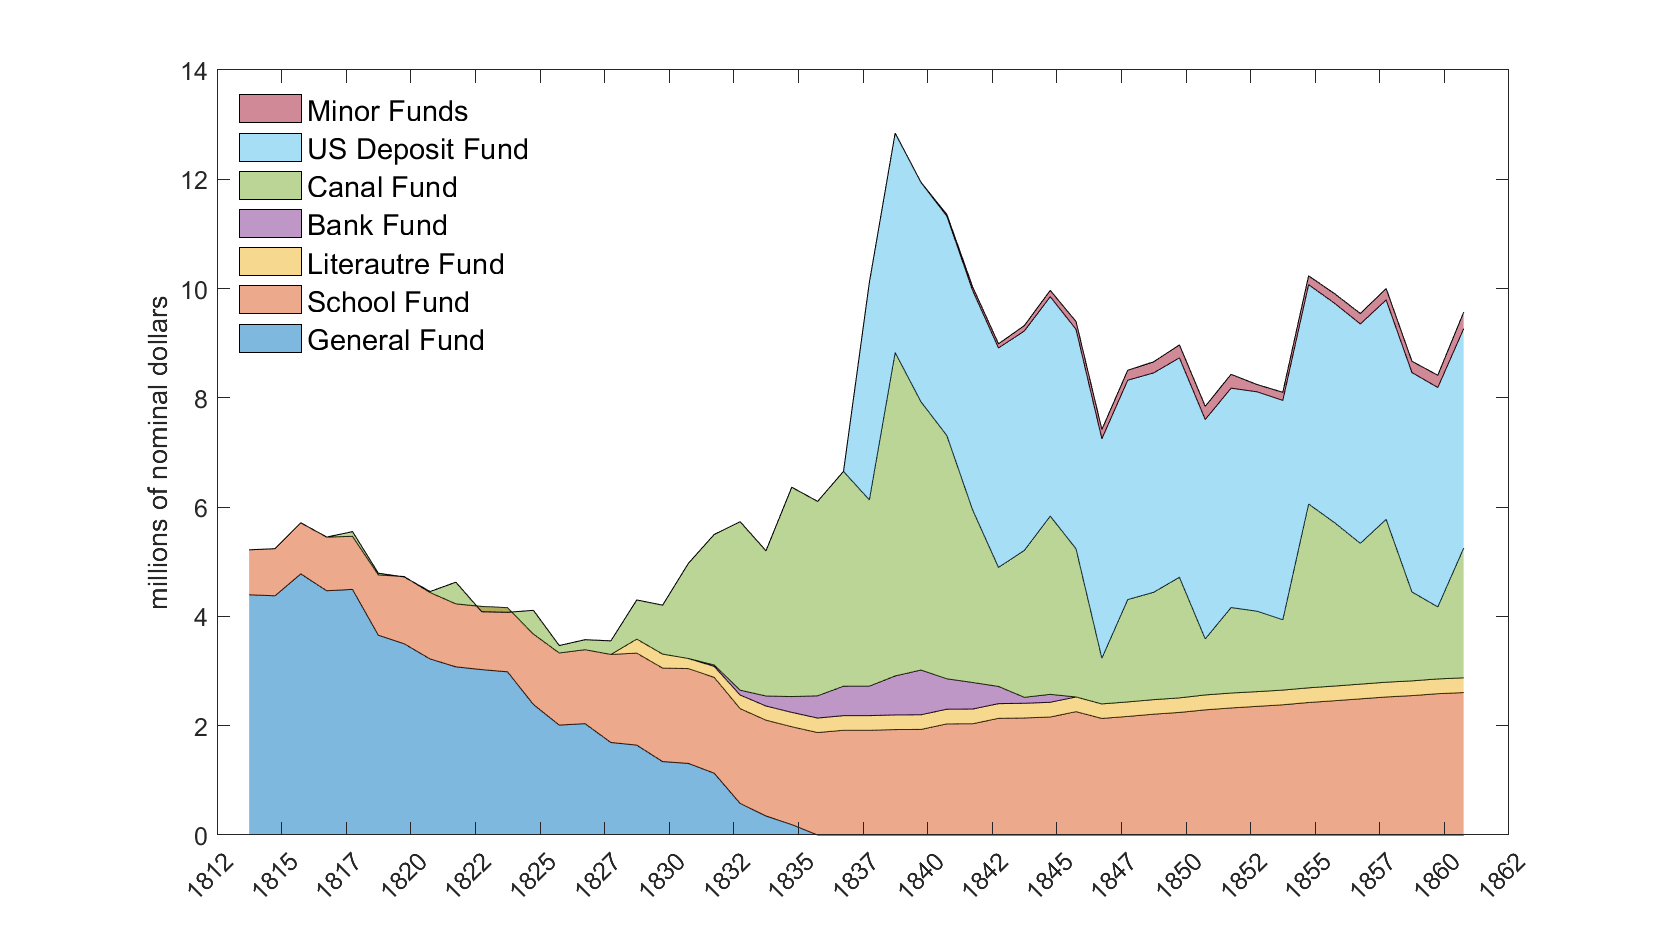
\includegraphics[scale=0.50]{fund_balances.png}}
\caption{New York State Fund Balances}
\label{fig:fund_balances}
\end{figure}

In figure~\ref{fig:fund_balances}, I plot the balances for these New York State funds.
In the remainder of this section, we discuss each of these funds in more detail.  These notes come from \citet{Roberts_1897} 
and various {\em Annual Reports of the Comptroller}.

\subsection{The General Fund}

\begin{itemize}

\item As can been seen in figure~\ref{fig:fund_balances}, in 1813, the General Fund balance was \$4.4 million.  
The income from the fund, together with receipts from salt and auction duties, was thought sufficient to 
maintain the operations of the State government.  


\end{itemize}


\subsection{The Common School Fund}

\begin{itemize}

\item In 1805, the Legislature used the proceeds from the sale of the first 
500,000 acres of vacant and unappropriated lands managed by the 
Surveyor-General to establish the {\em Common School Fund}, a permanent 
fund for the support of common schools.

\item This represented one of the earliest efforts by any American state to 
create an endowment explicitly dedicated to public education.  

\item Additional revenues were later added from various sources, 
and the fund grew from \$0.82 million in 1813 to \$2.6 million in 1860.
  
\item No direct state tax for school purposes was levied until 1853.  Thus, 
from 1805 to 1853, the interest of the Common School Fund, augmented by 
interest from the U.S. Deposit Fund (discussed below), was used to support 
the State’s system of free public education.  This policy reflected the early 
republican ideal that education, like government itself, might be sustained 
from the returns on public assets rather than from direct taxation.

\end{itemize}

\subsection{The Literature Fund}

\begin{itemize}

\item New York State Literature Fund was established in 1827 to support secondary education 
and the creation of libraries in academies, which were private schools for older students. 

\item Revenue for the Literature Fund came from various sources, including revenue from public lands 
and a small portion of the General fund.
    
\item Unlike the Common School Fund, which supported local, free-tuition elementary schools, 
the Literature Fund primarily supported 
academies, which typically charged tuition and catered to a wealthier class.

\item The Literature Fund was part of a larger state effort to provide public 
education. By funding libraries and teachers in academies, the fund promoted 
the study of literature and a broader curriculum beyond the basic literacy 
and moral instruction offered in the common schools. 
   
\item The Literature Fund was eventually consolidated with the United States Deposit Fund. 

\end{itemize}


\subsection{United States Deposit Fund} 


\begin{itemize} 

\item The United States Deposit Fund was created after the federal government distributed surplus federal funds to the states in 1837. 

\item The money in the fund was lent out by the state and was intended to be secured by real estate mortgages.

\item The interest generated from these loans was used to support the state's common school fund.

\end{itemize}


\subsection{The Bank Safety Fund}


\begin{itemize}

\item In 1829, New York State set up a bank insurance system called the {\em Bank Safety Fund.}

\item The system required banks to deposit securities in the Comptroller’s 
office as a guaranty for the notes issued by the banks.  It imposed annual 
assessments of 1/2 of 1\% of a bank's paid-in capital until each bank had 
paid in a total of 3\%. Banks were permitted to deposit up to 1/2 of their 
security in the form of bonds and mortgages.  

\item This fund would then be used to reimburse bank creditors in full, should a bank 
fail. These creditors were largely note holders.  Notes in circulation were 
twice the size of deposits at a typical bank.

\item Albert Gallatin noted:
\begin{quote}
... with the laudable intent to protect the community against partial
failures, a 'safety fund' has been established by law ... which is applicable
to the payments of the notes of any that may fail. This must
have the tendency to encourage excessive issues of paper, which could not be
sustained if resting only on the credit of the bank by which
they are made.
\end{quote}
Cite \cite{Bodenhorn_1996} for this quote.

\item There was also a bank supervision aspect to the system.  The 
legislation creating the system authorized the appointment of three Bank 
Commissioners charged with visiting and examining the banks and reporting to 
the Legislature.  The law also required every banking association to file 
semi-annual reports of its transactions with the Comptroller. 

\item Between February 1840 and October 1842, 11 banks failed.  These banks 
are listed in table~\ref{table:failed_banks}. In 1839, the balance (I assume 
measured at its par value) in the safety fund was \$0.818 million. Part of 
the banks' deposits in the Bank Safety Fund were bonds and mortgages, which 
fell in value during this period, the market value of the fund fell at 
exactly the time the Comptroller needed to sell assets to reimburse bank 
creditors.

\item The total cost to fund for insuring the creditors for the 11 
banks was \$2.565 million.   The fund became insolvent in 1843.

\item The office of the Bank Commissioners was abolished in 1843, and the 
responsibility for bank supervision was transferred to the Comptroller. In 1851, a 
separate Banking Department was established.

\end{itemize}



\begin{table}[htbp]
\centering
\small
\begin{tabular}{lrrrrr}
                               &             &               &   Other      &  Receipts     &  Balance  \\
                               & Date of     & Notes         &   Debts      &  from Asset   &  Paid by \\
Failed Bank                    & Failure     & Redeemed      &   Paid       &  Sales        &   Fund \\
\hline
City Bank of Buffalo           & 2/1840      & \$317,107 &           & \$99,996 & \$217,111 \STRUT \\
Wayne County Bank              & 12/1840     &   113,131   &  \$16,078 &          & 129,209 \\
Commercial Bank \\
\hspace{.1in} of New York City & 9/1841      & 139,837   & 146,129   &  7,188   & 278,778 \\
Bank of Buffalo                & 11/1841     & 435,540   & 149,241   &          & 584,781 \\
Commercial Bank 
\hspace{.1in} of Buffalo       & 11/1841     & 186,861   & 424,515   &  5,000   & 606,376 \\
Commercial Bank 
\hspace{.1in} of Oswego        & 12/1841     & 163,162   &  78,352   &  2,392   & 239,122 \\
Watervliet Bank                & 3/1842      & 134,107   &  77,484   & 13,258   & 198,333 \\
Clinton County Bank            & 4/1842      &  71,896   & 156,257   &          & 228,153 \\
Bank of Lyons                  & 9/1842      &  52,898   & 40,053    &  3,761   &  88,990 \\
Lafayette Bank, NYC            & 2/1842      &   38      &           &          &      38 \\
Oswego Bank                    & 10/1842     &\\
Not specified                  &             &     725   &           &  6,482   &      \\
\hline
Total                          & \$1,615,302 & \$1,088,109 & \$138,077 & \$2,565,334 \STRUT \\
\end{tabular}
\caption{Payments Made by the Bank Safety Fund to Reimburse Creditors of the Failed Banks}
\label{table:failed_banks}
\flushleft{\footnotesize Source: \citet[page 332]{Chaddock_1910} and \citet[page 25]{Bodenhorn_1996}.} 
\end{table}


\subsection{Minor Funds}

These minor funds were the Mariner's Fund, Auburn and Rochester Sinking Fund, Tonawanda Railroad Company Sinking Fund, Hudson \& Berkshire Railroad Company Sinking Fund, Long Island Railroad Company Sinking Fund, Tioga Cola Iron Mining \& Manufactures Sinking Fund, and the Stockbridge Indians Fund. 

\section{New York State Debts}

In figure~\ref{fig:debt_balances}, I plot the quantity of New York State debt outstanding.

\begin{figure}
\center{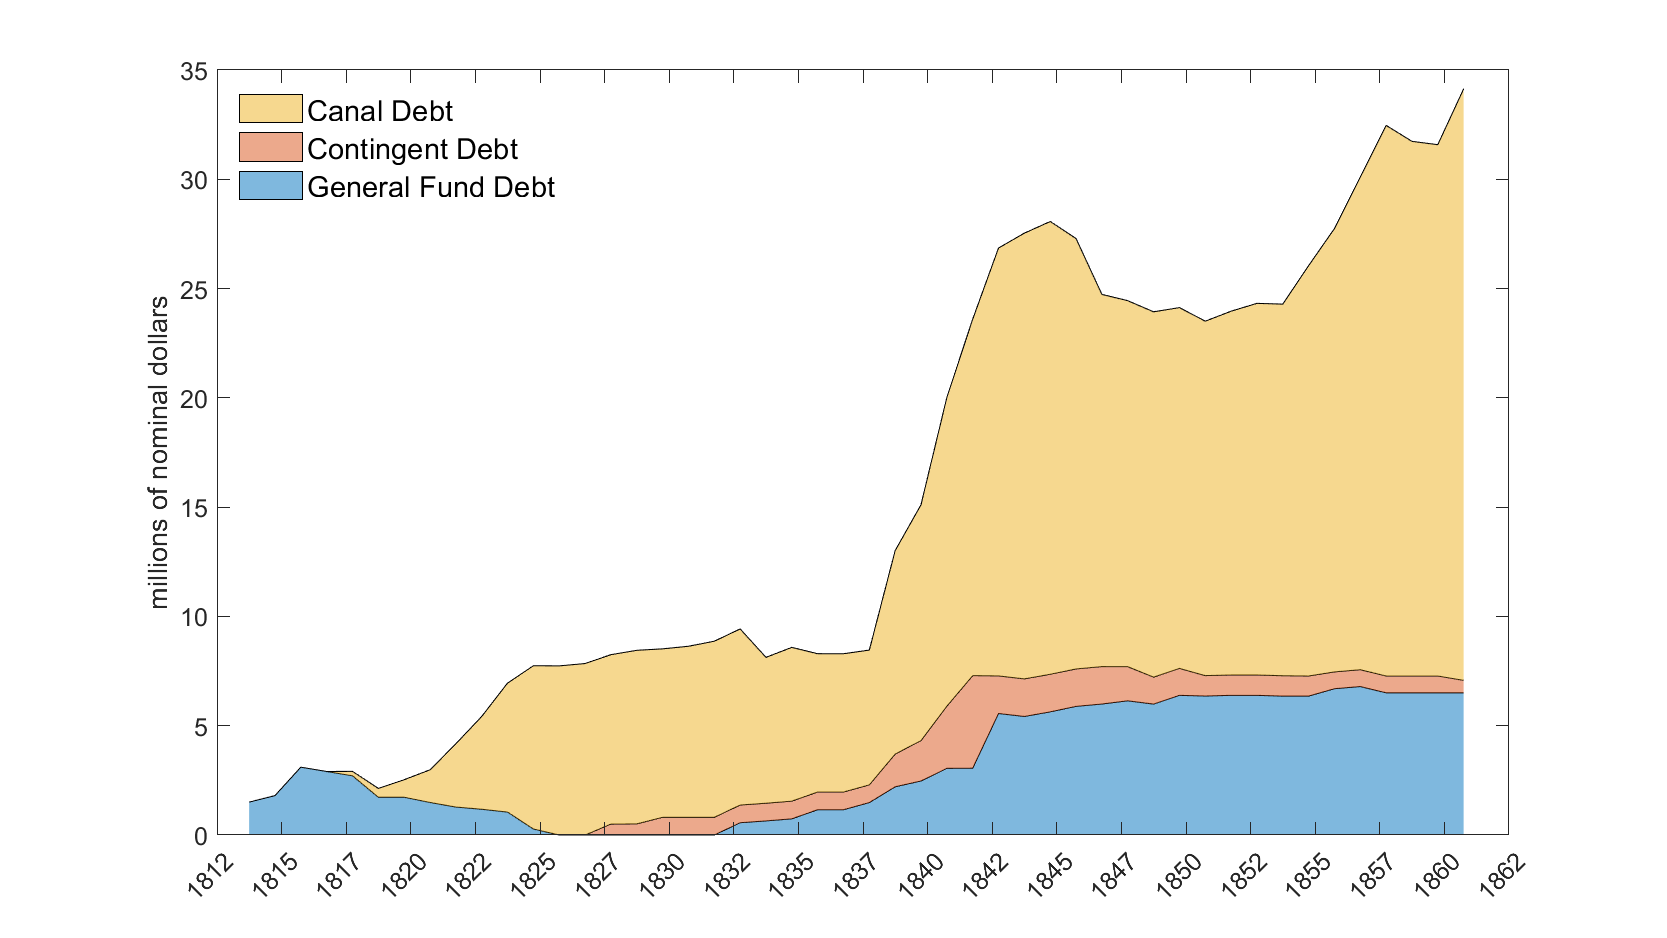
\includegraphics[scale=0.50]{debt_balances.png}}
\caption{New York State Debt}
\label{fig:debt_balances}
\end{figure}

\begin{itemize}

\item The three types of debt: General Fund debt, Contingent debt, and Canal debt.  Most of the debt issued by the New York was 
for the construction and maintenance of the Canal System.

\item About 42\% of the debt was held abroad. In table~\ref{table:ny_state_debt_1841_42} we reproduce a table from the 1842 Annual Report of the
Comptroller listing the bonds outstanding in 1841 and the distribution of their ownership.

\end{itemize}


\begin{table}[htbp]
\centering
\small
\begin{tabular}{lrrrr}
      & \multicolumn{3}{c}{Held}\\
      \cline{2-4}
Bond  & in New York &  in Other States  & by Foreigners & Total \STRUT \\
\hline
Erie and Champlain Canals         & \$150,529.98 & \$18,495.00 & \$1,715,412.23 & \$1,884,437.21\STRUT\\
Enlargement of Erie Canal         & 3,294,048.75 & 333,229.40  & 3,407,341.14   & 7,034,619.29 \\
Cayuga, Seneca, and Oswego Canals & 376,078.66   & 26,211.11   & 256,014.23     & 658,304.00 \\
Crooked Lake Canal                & 114,000.00   & ---         & 5,500.00       & 120,000.00 \\
Chemung Canal                     & 156,006.93   & 5,700.00    & 314,707.30     & 476,974.23 \\
Chenango Canal                    & 629,232.31   & 223,392.14  & 1,549,911.21   & 2,402,535.66 \\
Black River Canal                 & 357,551.82   & 8,166.67    & 739,954.74     & 1,105,673.23 \\
Genesee Valley Canal              & 606,063.82   & 81,905.00   & 1,878,411.00   & 2,566,379.82 \\
Oneida River Improvement          & 43,800.00    & 1,200.00    & 5,000.00       & 50,000.00 \\
Oneida Lake Canal                 & 50,000.00    & ---         & ---            & 50,000.00 \\
7 per cents of 1848               & 1,445,736.00 & 106,500.00  & 32,500.00      & 1,584,736.00 \\
7 per cents of 1849               & 1,608,000.00 & 13,600.00   & 31,000.00      & 1,652,600.00 \\
Delaware and Hudson Canal Co.     & 409,316.88   & 17,358.88   & 373,324.24     & 800,000.00 \\
New York and Erie Railroad Co.    & 2,587,000.00 & 251,000.00  & 162,000.00     & 3,000,000.00 \\
Tonawanda Railroad                & 86,000.00    & 14,000.00   & ---            & 100,000.00 \\
Schenectady Railroad              & 100,000.00   & ---         & ---            & 100,000.00 \\
Long Island Railroad              & 80,000.00    & 3,000.00    & 17,000.00      & 100,000.00 \\
Catskill and Canajoharie Railroad & 86,000.00    & ---         & 114,000.00     & 200,000.00 \\
Ithaca and Owego Railroad         & 82,000.00    & 12,000.00   & 221,700.00     & 315,700.00 \\
Auburn and Rochester Railroad     & 188,000.00   & 11,000.00   & 1,000.00       & 200,000.00 \\
Hudson and Berkshire Railroad     & 141,000.00   & ---         & 9,000.00       & 150,000.00 \\
Tioga Coal, Iron and Mining Co.   & 70,000.00    & ---         & ---            & 70,000.00 \\
Astor Stock                       & 561,500.00   & ---         & ---            & 561,500.00 \\
5 per cent Bank Fund Stock        & 350,257.00   & ---         & ---            & 350,257.00 \\
7 per cent stock and bonds        & 465,358.00  &  ---         & ---            & 465,358.00\\
\hline
Total                             & 14,038,540.15 & 1,240,962.10 & 10,833776.09 & 25,999,074.44\STRUT 
\end{tabular}
\caption{Ownership Distribution of New York State Debts, 1841--42}
\label{table:ny_state_debt_1841_42}
\flushleft{\footnotesize Source: 1942 {\em Annual Report of the Comptroller}, pages 9-10.}
\end{table}

\subsection{General Fund Debt}

\begin{itemize}

\item There is general fund debt in 1814 along with a positive balance in the General Fund.  This debt was paid off by 1825. 

\item In 1832, the State resumed borrowing to pay for ordinary expenditures.  The debt increases in the early 1840s as the government assumes the debts
of three failed railroads.  See the following subsection.


\item The Constitution of 1846 introduced a new fiscal framework.  It mandated the creation of a sinking fund for the gradual redemption of the General Fund debt.  
The management and investment of this sinking fund were entrusted to the Comptroller.  
The State retired the last of this debt in 1878.  

\end{itemize}


\subsection{Contingent Debt}

\begin{itemize}

\item Starting 1827, the State issued debt on behalf of various canal and 
railroad companies. While the companies were responsible for making the coupon 
and principal payments, the authorizing legislation ``pledges the faith and 
credit of this State for the payment of the interest and principal" on these 
bonds. These guarantees were backed by mortgages on the railroad and 
property.

\item The coupon and principal payments were payable in London. (source is a Comptroller report in the early 1840s.  Find it.)

\item These debts were called {\em contingent debt}. They were implicit liabilities of the State.

\item On July 1, 1841, the Ithaca and Owego, and Catskill and Canajoharie 
railroads stopped making their coupon payments. At a later date (find this 
date), the New York and Erie railroad defaulted as well. Consequently  
\$3,315,700 in railroad debt became State obligations and part of the General 
Fund debt.  This can be seen in figure~\ref{fig:debt_balances} as between 
1841 and 1842, the contingent debt drops by \$2,515,700, and the General 
Fund debt increases by  \$2,503,324.14. There is an extra \$1 million that 
must be ``netted out" somehow.  I need to figure this out.


\end{itemize}


\subsection{Canal Debt}

The Canal debt makes up the lion's share of the debt.  It increased in early late 1810s and early 1820s as well as the early 1840s.  These increase correspond to construction periods.

\newpage

\section{The Canal Account}

In figures~\ref{fig:canal_revenue}, \ref{fig:canal_outlays}, and ~\ref{fig:canal_rev_out}, we plot the Canal Account's revenues and expenditures.

\begin{itemize}

\item In figure~\ref{fig:canal_revenue}, we see that from 1817 to 1820, taxes were the sole source of revenue.  These were taxes on auctions, salt, and steamboat revenue.  Between 1817 and 1836, these taxes were diverted from the General Account to the Canal Account.

\item While the Erie Canal officially opened on October 26, 1825, the Canal started to collect toll revenue in 1821 and by the late 1820s, it became the largest share of revenue.    Revenues declined in the late 1830s and in the 1850s.

\item In figure~\ref{fig:canal_outlays}, we see that there are spikes in outlays due to the construction of new branches. 
 
\item In figure~\ref{fig:canal_rev_out}, we see a form of the "law of gravity" between outlays and revenues.  I net out transfers to and from the General Fund in this figure.  
    
\end{itemize}


\begin{figure}
\center{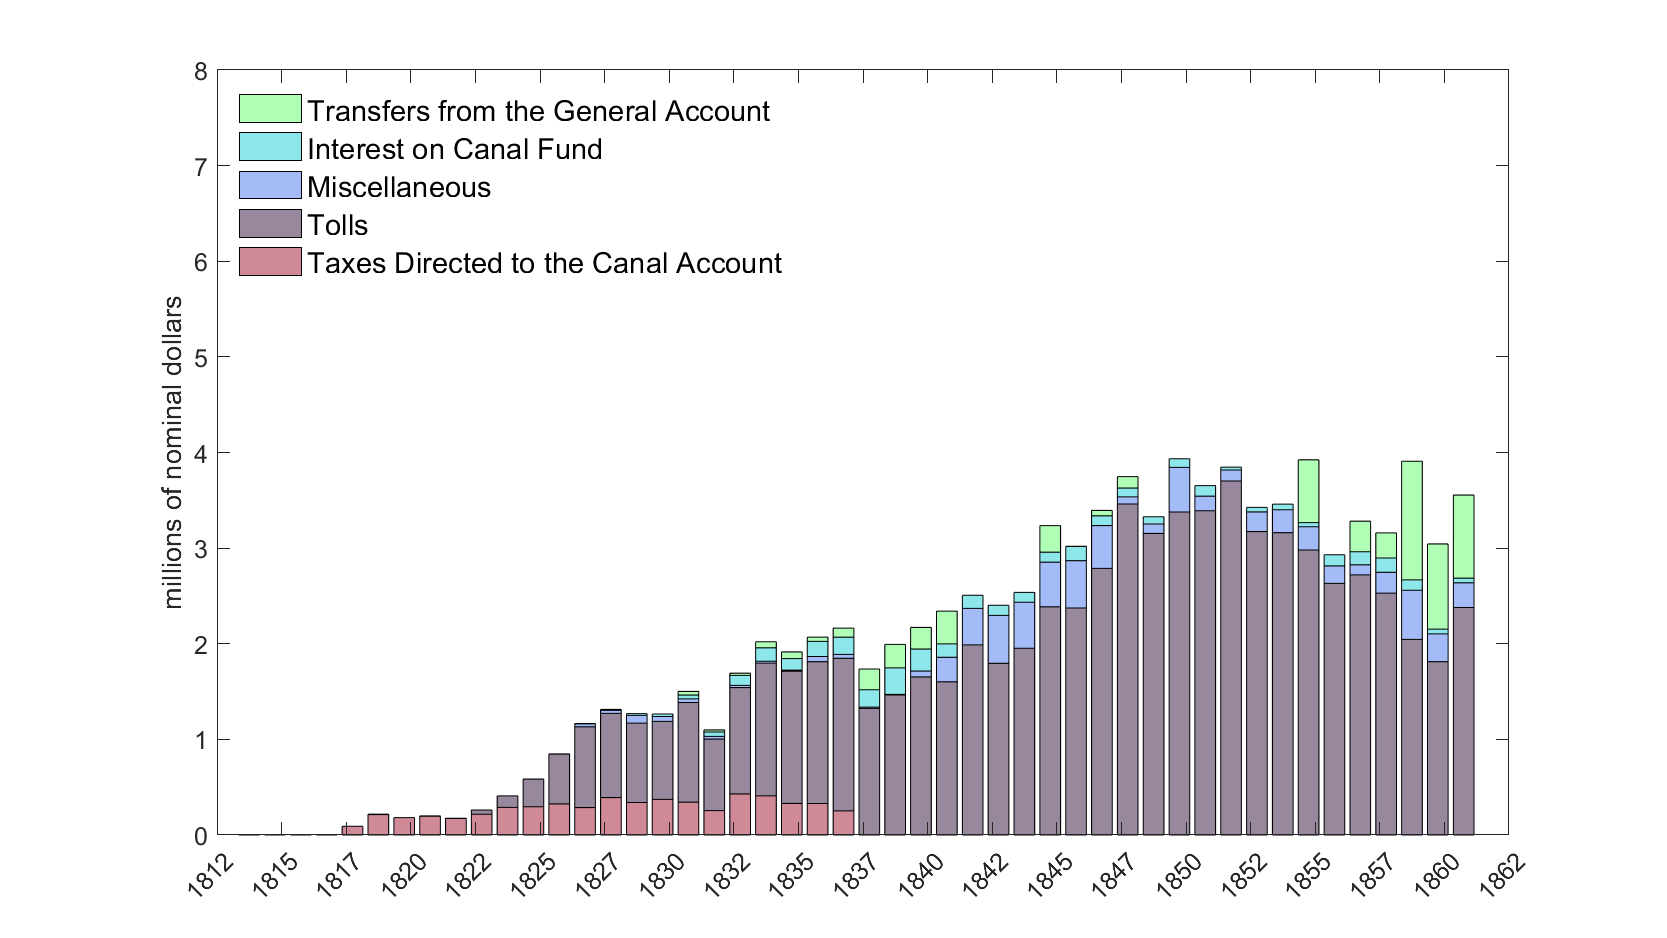
\includegraphics[scale=0.50]{canal_account_revenue.png}}
\caption{Canal Account Revenues}
\label{fig:canal_revenue}
\end{figure}


\begin{figure}
\center{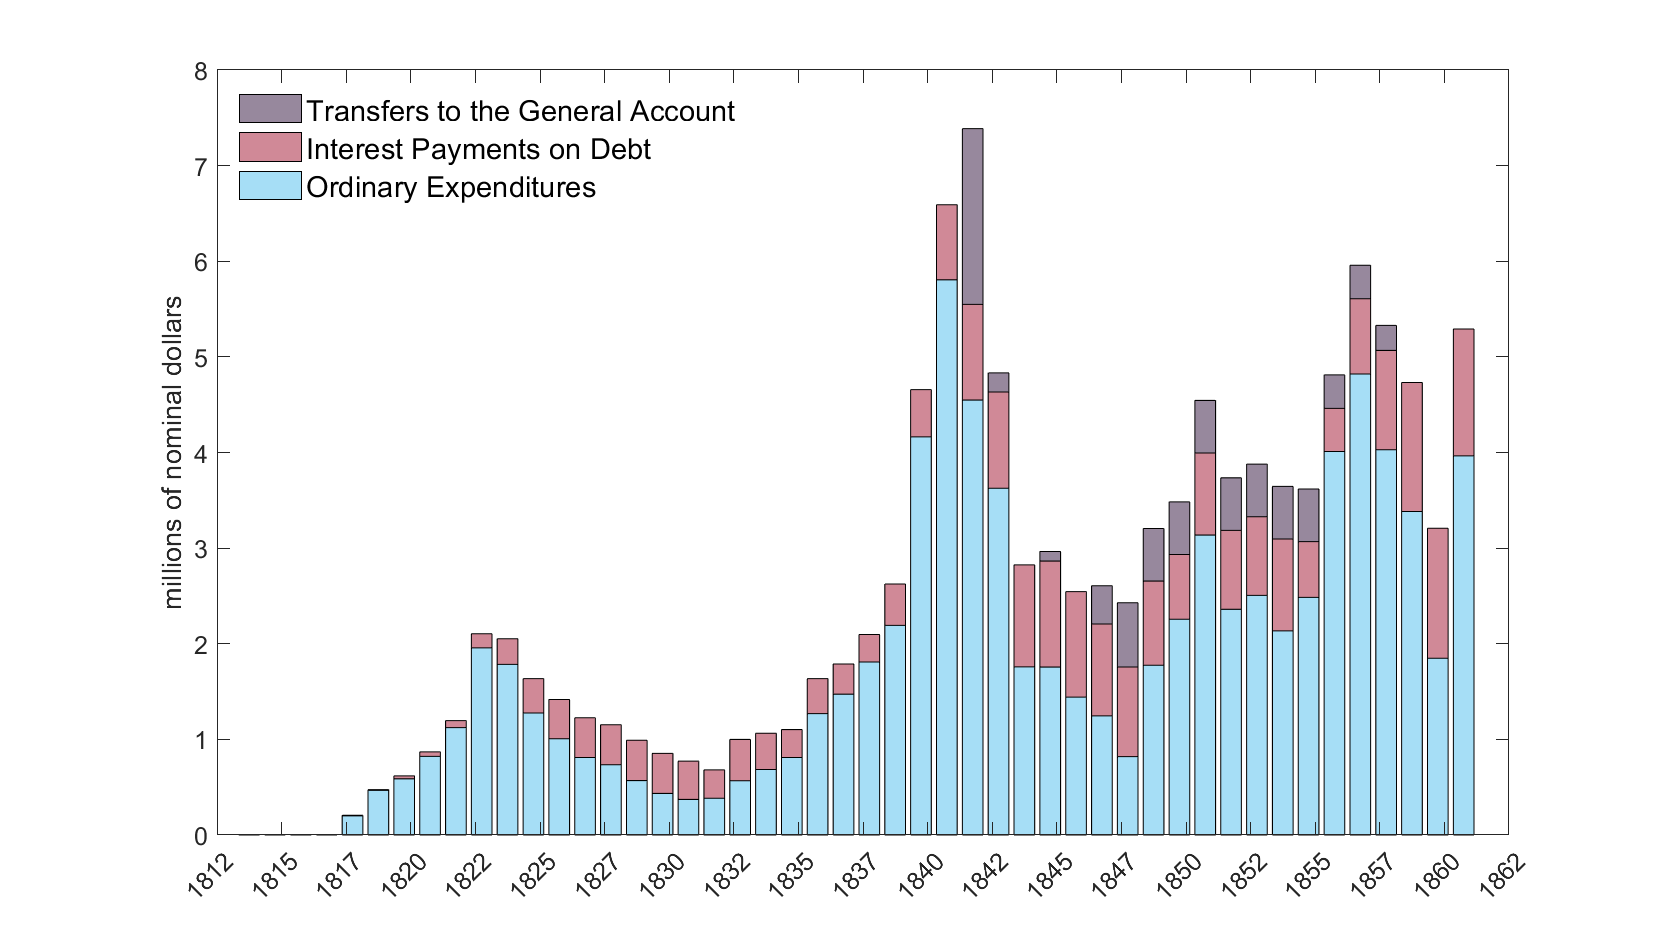
\includegraphics[scale=0.50]{canal_acct_spending.png}}
\caption{Canal Account Expenditures}
\label{fig:canal_outlays}
\end{figure}


\begin{figure}
\center{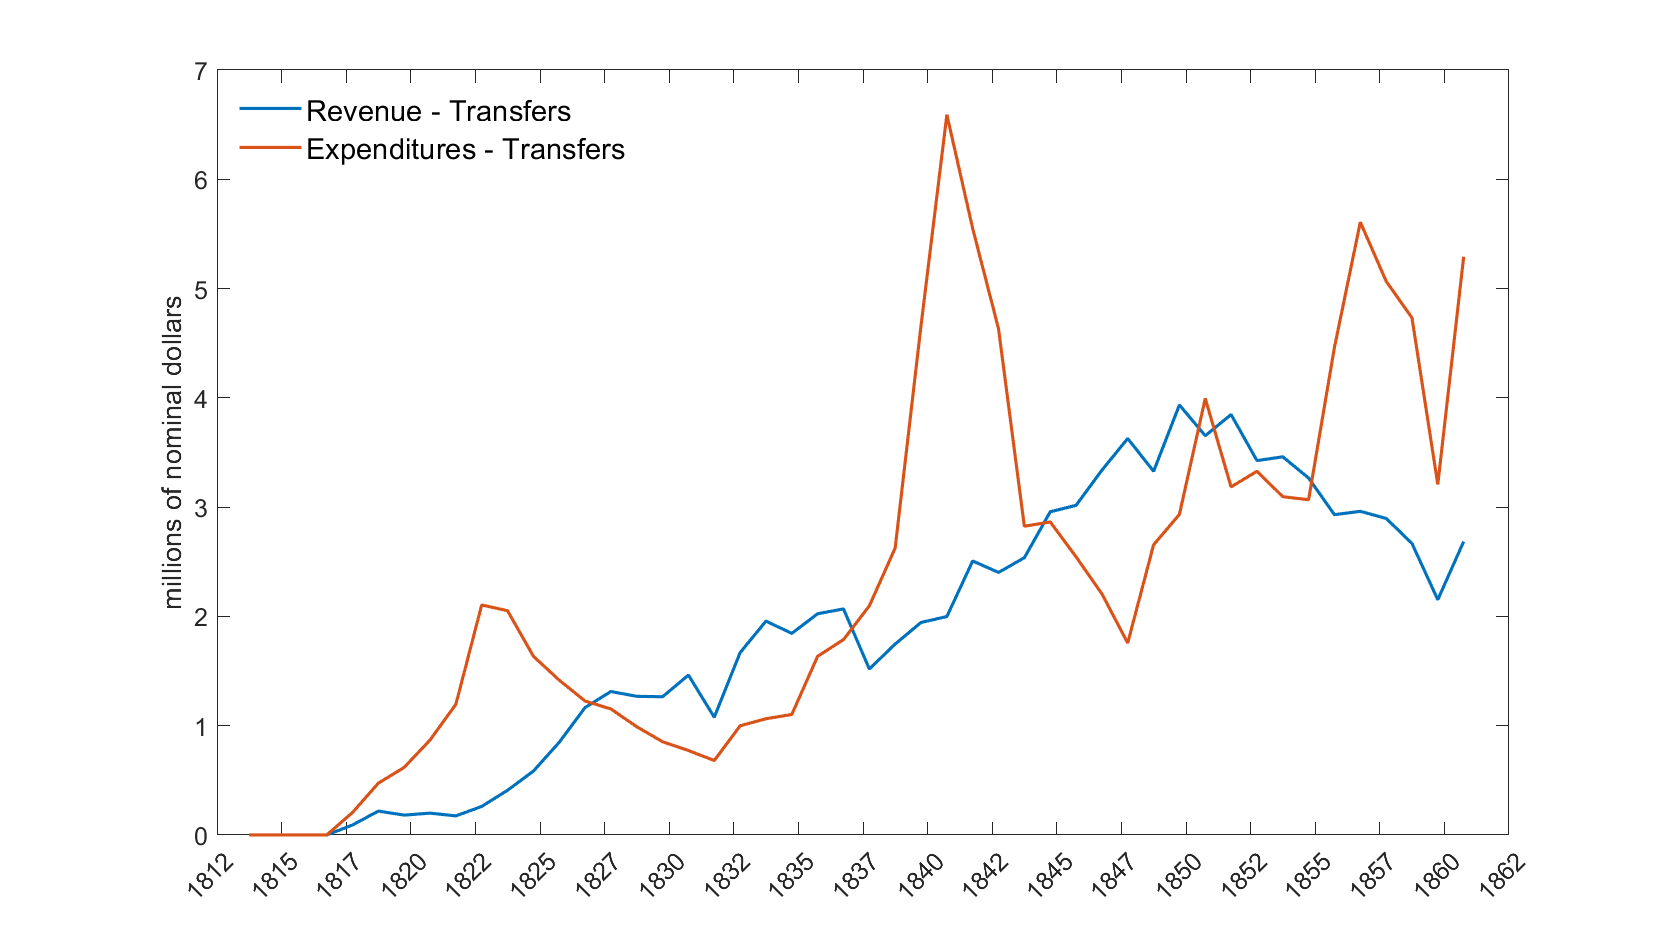
\includegraphics[scale=0.50]{erie_canal_revenue_outlays.png}}
\caption{Canal Account Revenue and Expenditures}
\label{fig:canal_rev_out}
\end{figure}

In figure~\ref{fig:canal_transfers} I plot transfers between the Canal Fund 
and the General Fund.  Prior to 1840, the Canal received transfers from the 
General Fund. After 1840, the flows went the other way.


\begin{figure}
\center{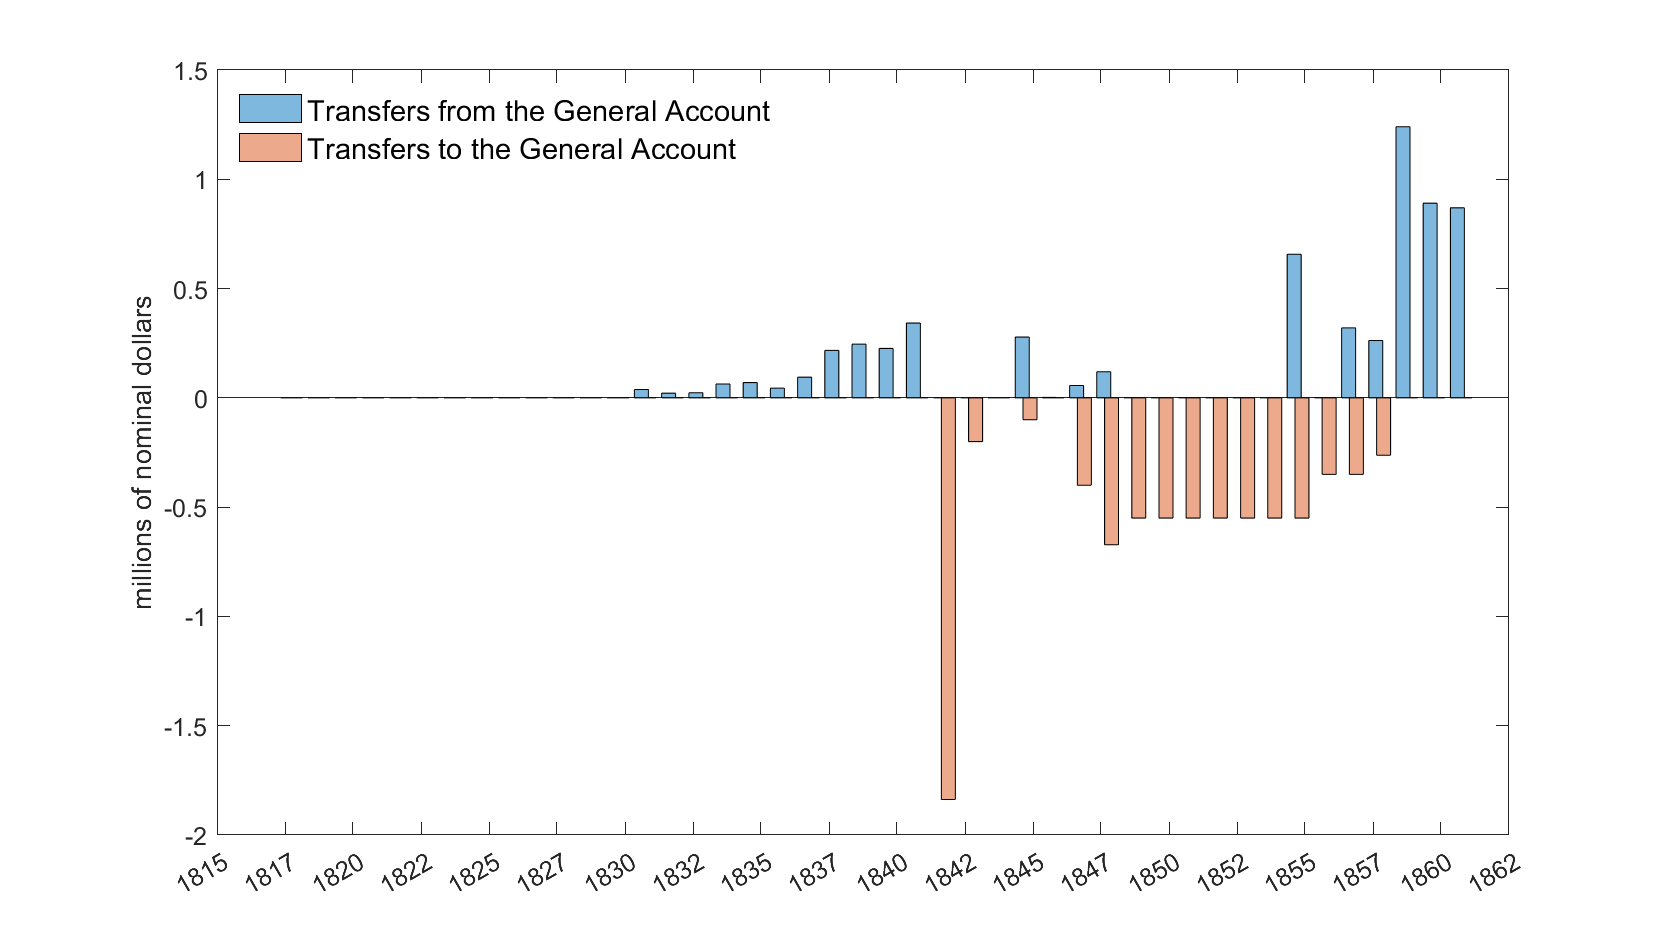
\includegraphics[scale=0.50]{erie_canal_transfers_tofrom_general_fund.png}}
\caption{Transfers Between the Canal  Accounts and the General Account}
\label{fig:canal_transfers}
\end{figure}

The New York Canal System generated a tremendous amount of economic growth for the state. 
I don't have any data to support this, but it is clear that the New York State economy grew during this period.
Ideally, I would plot these series as ratios of state GDP.




\section{The General Account}

\begin{itemize}

\item In figure~\ref{fig:general_acct_revenue}, I plot the sources of General Account revenues from 1813 to 1860
\begin{itemize}
\item Land sales make up a relatively small share of total revenue

\item During the late 1820s and early 1830s, revenue from the state accounts made up the lion's share of revenue.  In 1832, the State resumed borrowing to pay for ordinary expenditures. 

\item A state property tax was in effect between  1816 and 1826, which accounted for a large share of revenue.  The property tax was reinstated in 1842.

\item The large payment from the federal government is the distribution of the federal surplus to the states mandated by the Deposit Act of 1836.

\end{itemize}

In figure~\ref{fig:general_acct_outlays}, I plot expenditures over time.
\begin{itemize}

\item Ordinary expenditures peak during the War of 1812 and then decline.  They generally rise over time.  I don't scale by population or by output.

\item The assumption of the contingent debt from the three failed railroads (in purple) in 1841 and 1842 stands out.

\item The insurance payments to the creditors of the failed banks also raised expenditures in the early 1840s.

\end{itemize}

In figure~\ref{fig:general_acct_rev_out} we plot General Account revenue and expenditures (net transfers) on a single figure.  Before the early 1830s, the General Account's budget was balanced.  In the 1840s and 1850s, the General Account ran deficits.


\end{itemize}


\begin{figure}
\center{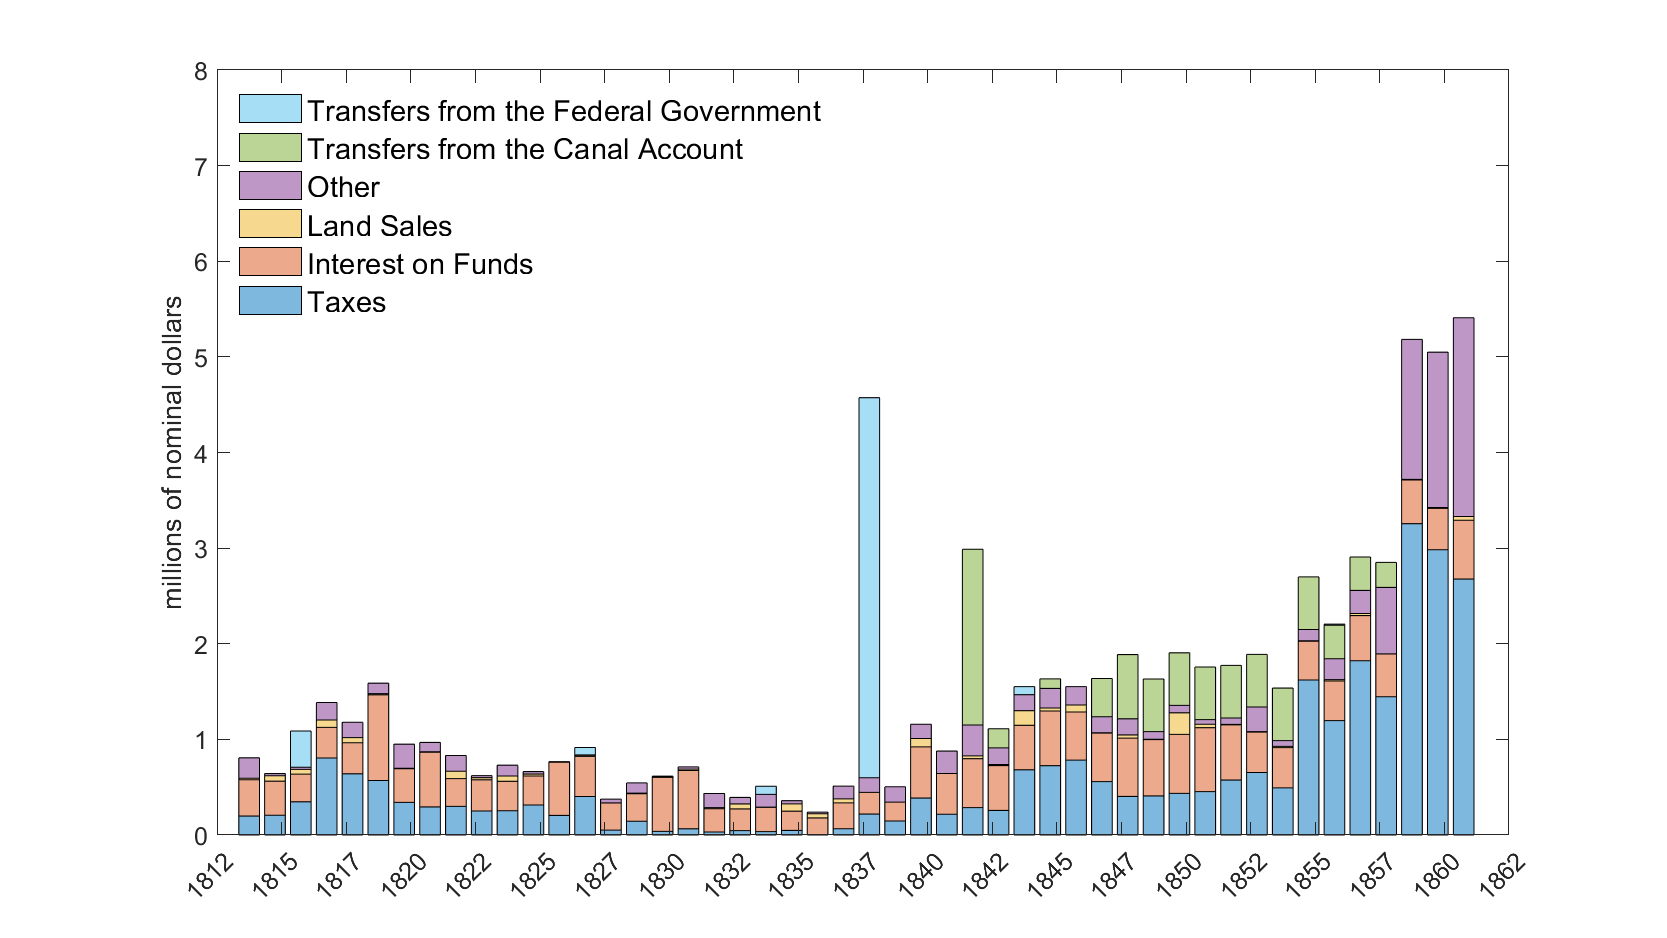
\includegraphics[scale=0.50]{general_account_revenue.png}}
\caption{General Account Revenues}
\label{fig:general_acct_revenue}
\end{figure}


\begin{figure}
\center{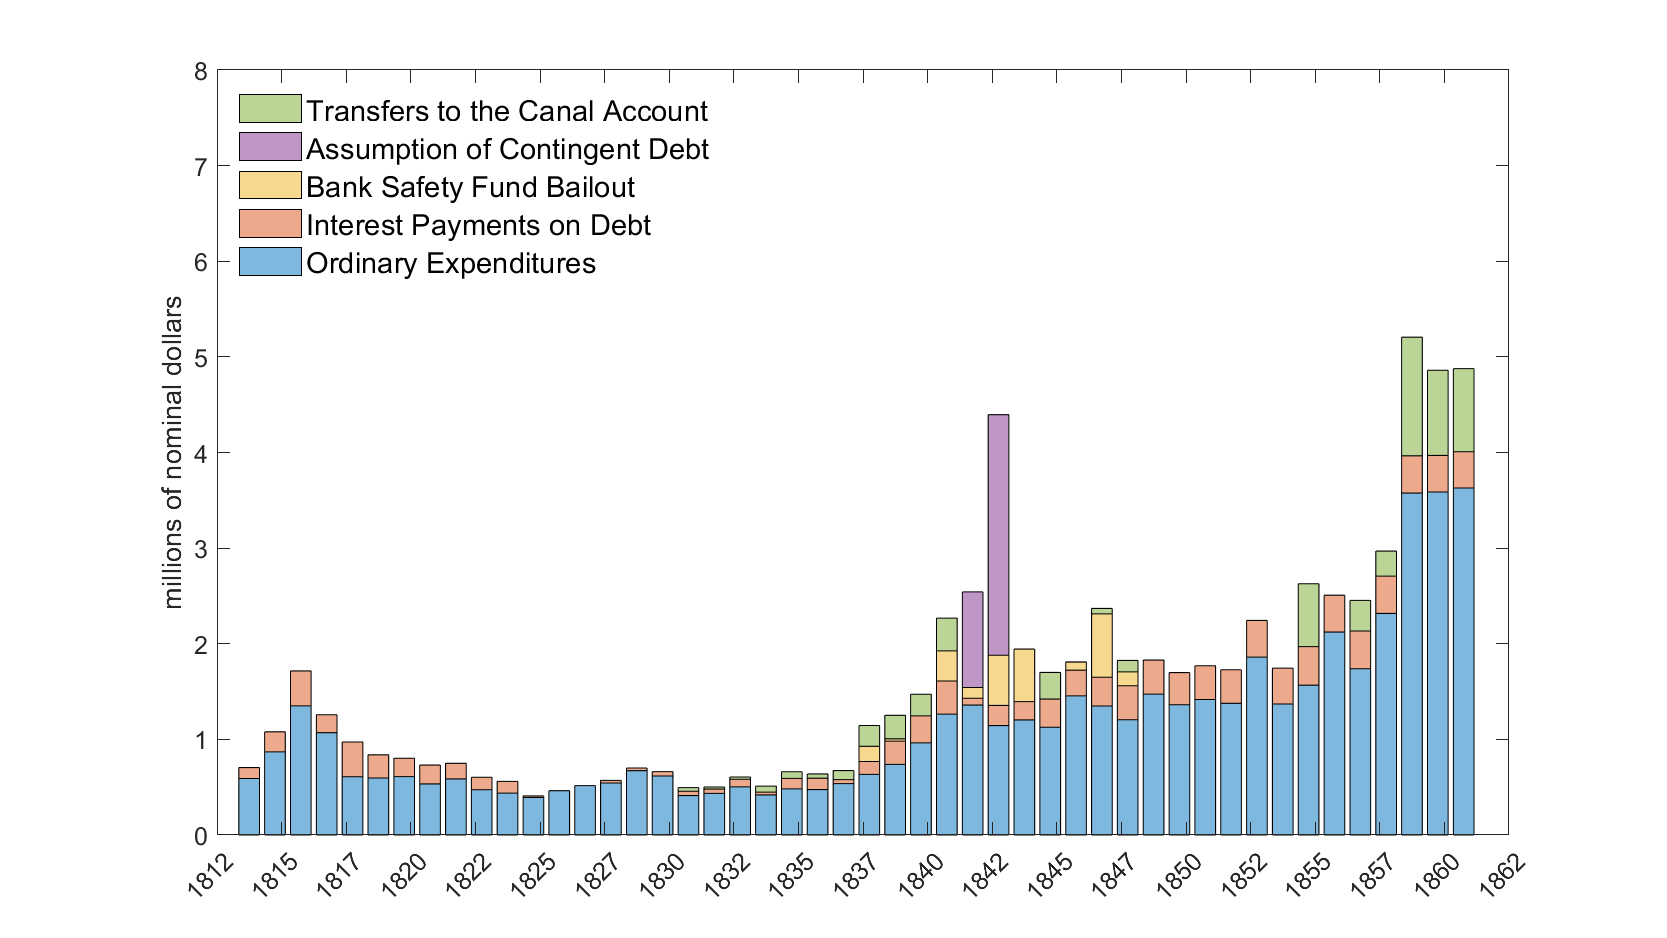
\includegraphics[scale=0.50]{general_acct_spending.png}}
\caption{General Account Expenditures}
\label{fig:general_acct_outlays}
\end{figure}


\begin{figure}
\center{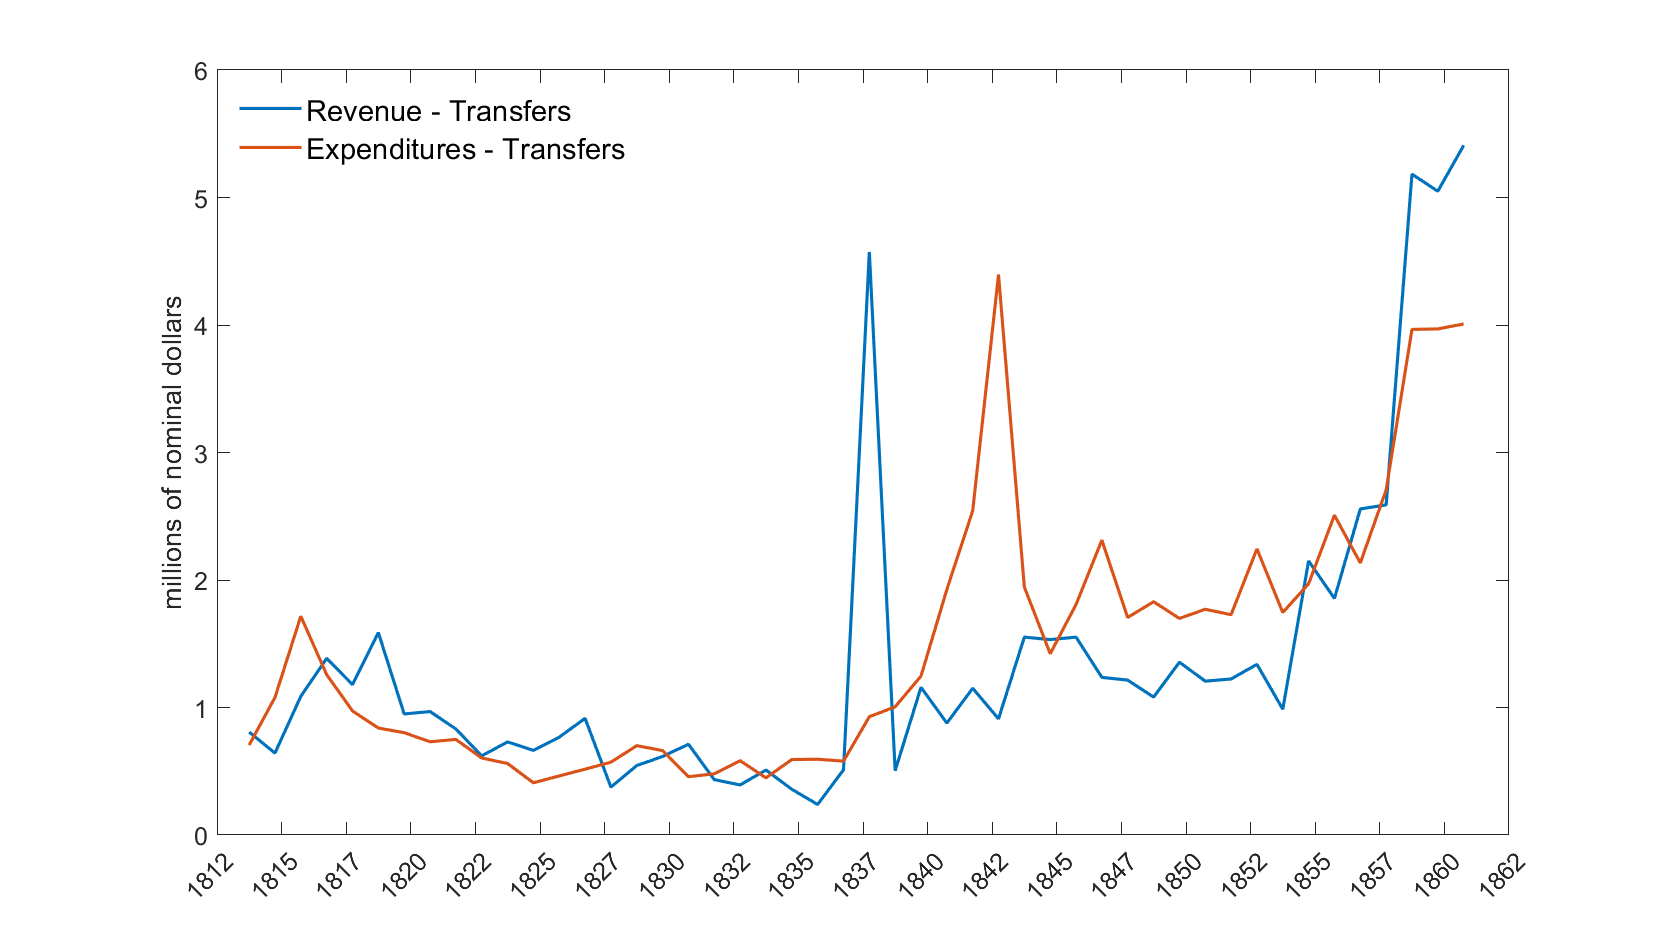
\includegraphics[scale=0.50]{general_acct_revenue_outlays.png}}
\caption{General Account Revenue and Expenditures}
\label{fig:general_acct_rev_out}
\end{figure}


\section{Consolidated Accounts}

In figures~\ref{fig:consolidated_revenue}, \ref{fig:consolidated_outlays}, and ~\ref{fig:consolidated_rev_out}, we plot 
the merged Canal and General Account's revenues and expenditures.

\begin{itemize}

\item The Canal Account's revenues and expenditures are far larger than those of the General Account.  New York State is 
primarily a canal operator with a secondary role in general government.
    
\item With the big exception of the late 1830s and early 1840s, the consolidated budget is largely balanced over this time period.
 
\end{itemize}    


\begin{figure}
\center{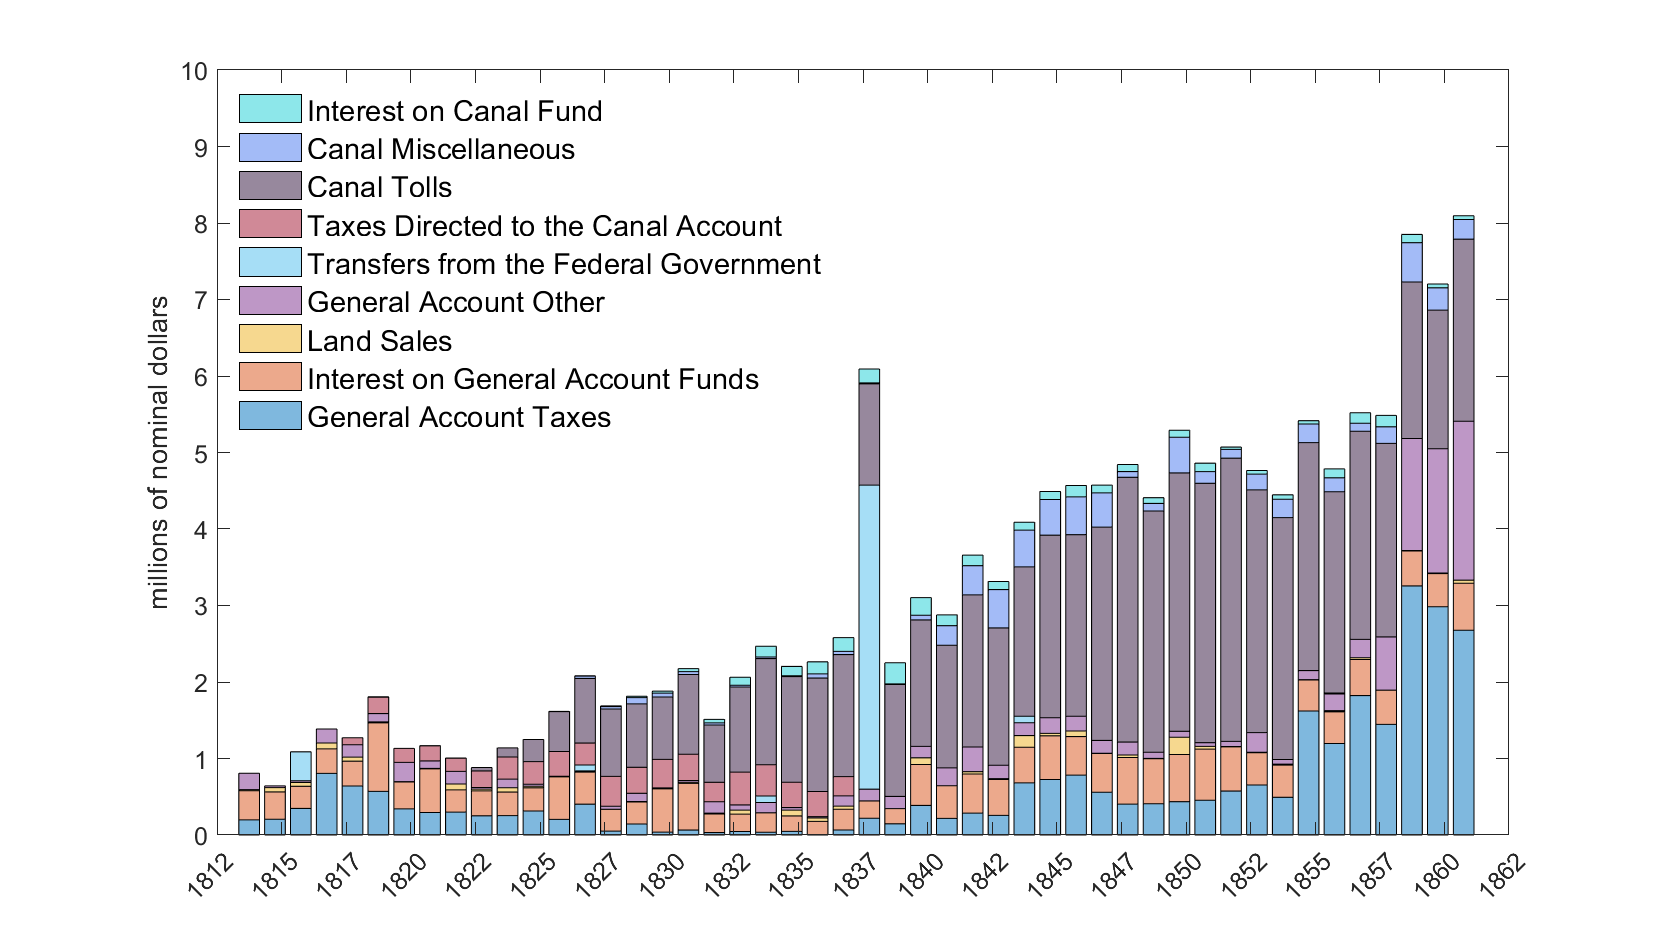
\includegraphics[scale=0.50]{consolidated_account_revenue.png}}
\caption{Consolidated Revenues}
\label{fig:consolidated_revenue}
\end{figure}


\begin{figure}
\center{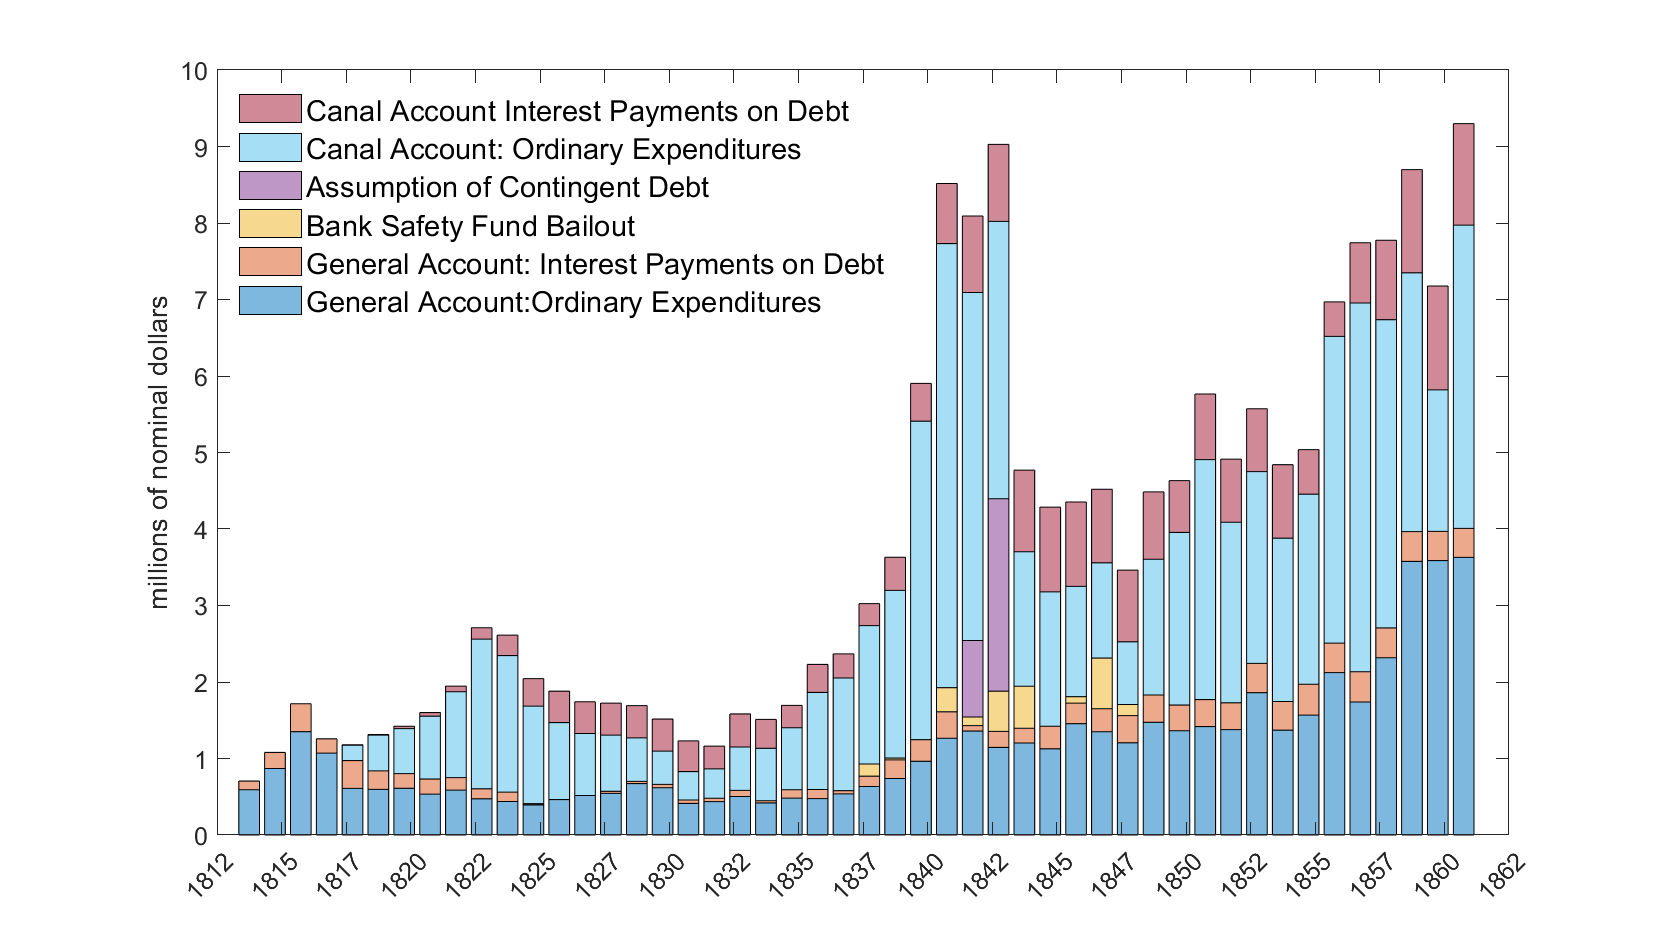
\includegraphics[scale=0.50]{consolidated_acct_spending.png}}
\caption{Consolidated Expenditures}
\label{fig:consolidated_outlays}
\end{figure}


\begin{figure}
\center{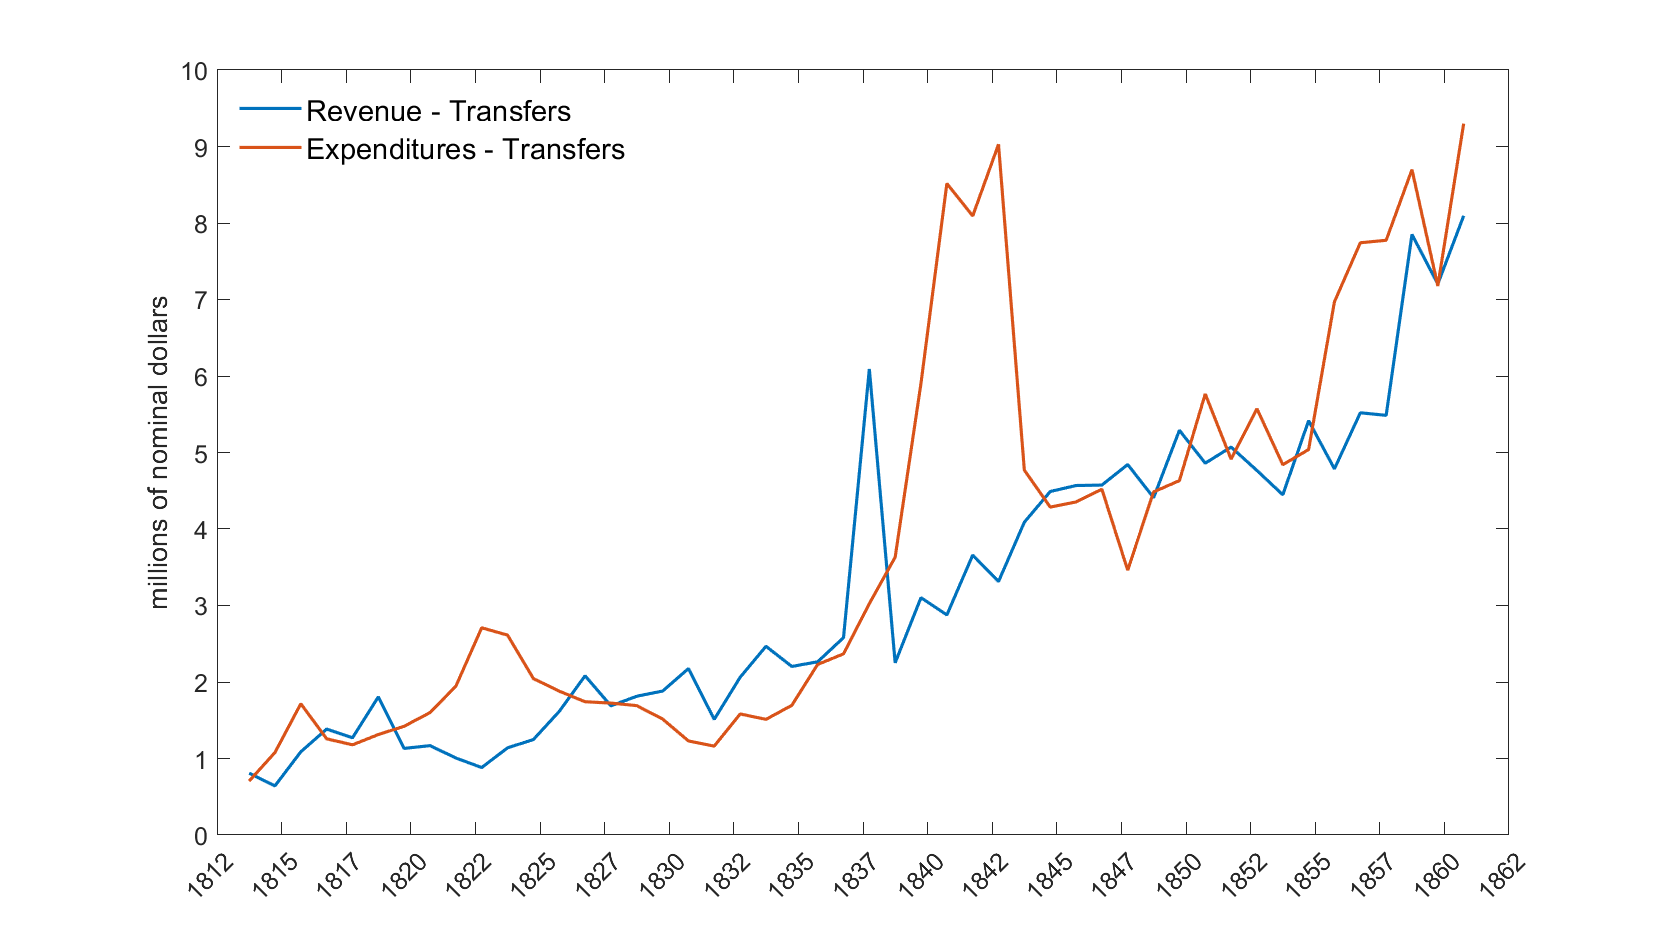
\includegraphics[scale=0.50]{consolidated_revenue_outlays.png}}
\caption{Consolidated Revenue and Expenditures}
\label{fig:consolidated_rev_out}
\end{figure}

\newpage

\section{Bond Prices}

\begin{figure}
\center{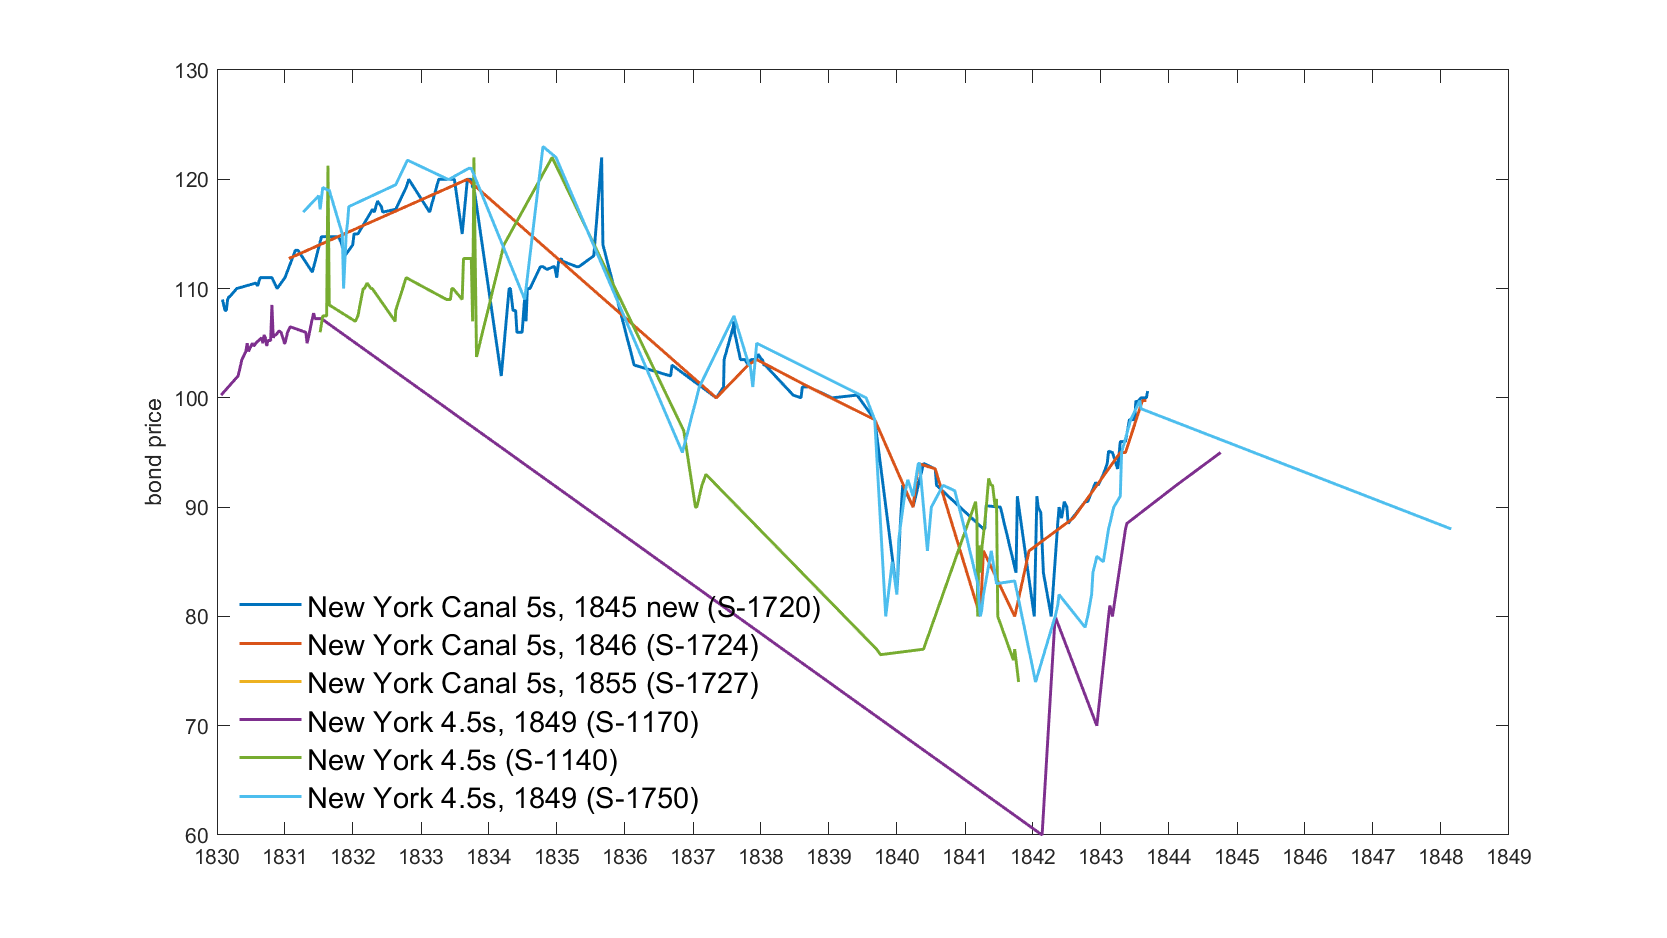
\includegraphics[scale=0.50]{ny_state_debt_prices.png}}
\caption{Prices of Various New York State Bonds}
\flushleft{\footnotesize Source: \cite{Sylla_Wilson_Wright}.}
\label{fig:nys_bond_prices}
\end{figure}

\begin{itemize}

\item In figure~\ref{fig:nys_bond_prices} I plot the prices of three Canal bonds and three General Fund bonds.  

\item The late 1830s and the early 1840s were a period of fiscal stress for New York. During this period, the Legislature suspended all public works except those whose suspension would result in a significant loss and pledged the state's revenues for the payment of its obligations. It is hard to see this ``suspension" in the Canal Account expenditures, figure~\ref{fig:canal_outlays}.

\item Despite never missing a coupon and principal payment, New York State bond traded at 80 cents on the dollar in the early 1840s. The Comptroller complains about this.

\item I should convert prices to yields.

\end{itemize}


\section{Unit of Account Issues}

The source for this section is \cite{Roberts_1897}.

\begin{itemize}

\item When specie payments 
were suspended during the financial panic of 1837, Comptroller Azariah C. 
Flagg used State resources to make up the difference between depreciated 
paper currency and coin to honor the State’s obligations at par.  

\item In 1857, Comptroller William F. Allen likewise urged that the State’s bonded debt be 
serviced in coin rather than in paper arguing that the 
public faith of New York should not fluctuate with the market value of its 
currency.

\item During the Civil War, when specie commanded a substantial premium over paper 
currency, the State of New York faced the question of whether its own bonded 
obligations should be paid in coin or in depreciated legal-tender notes.  In 
1863 and 1864, Comptroller Lucius Robinson recommended that both the 
principal and the interest on the State’s bonded debt be paid in specie.  The 
The legislature declined to follow his advice.

\item Although the Legislature again deferred action, the policy eventually 
prevailed.  In 1870, the State entered the open market and purchased coin to 
pay interest on its outstanding bonds.  This practice was continued until the 
general resumption of specie payments by the Federal Government in 1879.  

\item By adhering voluntarily to a metallic standard during the years of national paper 
currency, New York strengthened its standing in credit markets and set a 
precedent for conservative financial management that endured well into the 
late nineteenth century.

\end{itemize}

\section{Data Sources}

\begin{itemize}

\item The data for revenues and expenditures for the General Account are from Appendices I and II of \cite{Sowers_1914} and the 
{\em Annual Report of the Comptroller} for the State of New York.  The decomposition of General Fund revenues is from Sower.  

\item Data on the debt outstanding, fund balances, and Treasury balances are from the {\em Annual Report of the Comptroller}.

\item The Canal Account revenues, expenditures, debt outstanding, and fund balances are from Table No 82 on page 88 of the 1860
{\em Annual Report of the Commissioners of the Canal Fund to the Legislature of the State of New York}.

\item Unlike other state fiscal datasets, our records are consistent with the budget constraints presented at the start of this memo.

\end{itemize}


\clearpage
\bibliography{war_finance}

\end{document}

